\chapter{Eulerian Paths and Cycles}

Ajur was still tired after listening to so many definitions and examples the day before. He complained to Jura that their recent conversation with Rishnak was too similar to a boring math class. He said, ``I prefer to solve problems that are fun.''

Rishnak was near and overheard Ajur. Sighing, Rishnak did agree that the previous day's exchanges were dry. His ghost friends were right---he was making the beautiful subject of graph theory dull and monotonous. So for the next session, Rishnak decided to reach Ajur a more interesting problem, the existence of an Eulerian \index{Eulerian Walk}  walk.

Recall that a connected graph is a graph in which there is a path between every possible pair of vertices. Given this, an \textit{Eulerian walk} in a connected graph is a walk that includes every edge exactly once. This is also known as an \textit{Eulerian path} and this path can visit vertices more than once if need be. If the starting vertex and the ending vertex are the same then the walk is called a \textit{closed Eulerian walk} or an \textit{Eulerian cycle}. The problem is named in honor of Leonhard Euler, the first person to describe this (in the 1700s!).

The question of whether or not a given connected graph has an Eulerian walk (or a closed Eulerian walk) is among the oldest problems in graph theory. ``Ajur will love this problem,'' thought Rishnak as he searched for Ajur in the cemetery.

It did not take long for Rishnak to catch up with Ajur and Jura as they walked along a desolate path in a far corner of the cemetery.

Rishnak flashed his hands to produce a new graph [Figure~\ref{4g1}], then asked Ajur, ``In this graph, is there a walk starting from vertex~2 and ending at vertex~4 that travels through all of the edges \textit{exactly once}?''

\begin{figure}
\begin{center}
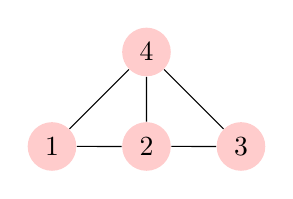
\begin{tikzpicture}
  [scale=.6,auto=left,every node/.style={circle,fill=red!20}]
  \node (n1) at (1,7) {1};
  \node (n2) at (3,7)  {2};
  \node (n3) at (5,7)  {3};
  \node (n4) at (3,9)  {4};

  \foreach \from/\to in {n1/n2,n2/n3,n2/n4,n1/n4,n3/n4}
    \draw (\from) -- (\to);

\end{tikzpicture}
\caption{Example graph with four vertices and five edges}\label{4g1}
\end{center}
\end{figure}

Ajur studied the graph, frowning.

Rishnak continued, ``If you find one, know that it is called an Eulerian walk. This is just like asking if you can trace all the edges once and only once without lifting your pen---or your stick.''

Ajur noticed that there was a cycle.  ``I see the cycle $(2,3,4,1)$ and after this cycle, we're back at vertex~2 with just one edge left, the edge $(2,4)$.  Can we visit a vertex more than once?''

Rishnak nodded.

Jumping up, Ajur grabbed a stick and drew a graph in the dirt [Figure~\ref{4g15}], using arrows to show how he traversed the edges with vertex~2 as the starting point. ``There's an Eulerian walk by combining the cycle and that last remaining edge. The path is $2-(2,3)-3-(3,4)-4-(4,1)-1-(1,2)-2-(2,4)-4$ or just $(2,3,4,1,2,4)$ with edges omitted.''

\begin{figure}
\begin{center}
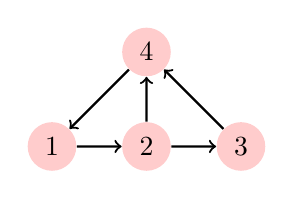
\begin{tikzpicture}
  [scale=.6,auto=left,every node/.style={circle,fill=red!20}]
  \node (n1) at (1,7) {1};
  \node (n2) at (3,7)  {2};
  \node (n3) at (5,7)  {3};
  \node (n4) at (3,9)  {4};

\path [->,draw,thick]
(n2) edge  (n3)
(n3) edge   (n4)
(n4) edge   (n1)
(n1) edge   (n2)
(n2) edge  (n4)
;
\end{tikzpicture}
\caption{Eulerian walk $(2,3,4,1,2,4)$ from vertex~2 to vertex~4 of the graph shown in Figure~\ref{4g1}}\label{4g15}
\end{center}
\end{figure}

Rishnak nodded again.  ``This is an Eulerian walk. If we were able to start and end on the same vertex, it would be a closed Eulerian walk.''

Ajur smiled. ``I see. So there is no closed Eulerian walk in this graph because that would necessarily imply that every vertex had even degree!''

Rishnak also smiled.  ``That's correct, Ajur.''

In a flash of light, Rishnak showed Ajur another graph [Figure~\ref{4g2}] and said, ``Here's a more challenging problem for you. In this graph, is there a walk from vertex~1 that ends at vertex~9 and traverses every edge exactly once?  In other words, is there an Eulerian walk from vertex~1 to vertex~9?''

\begin{figure}
\begin{center}
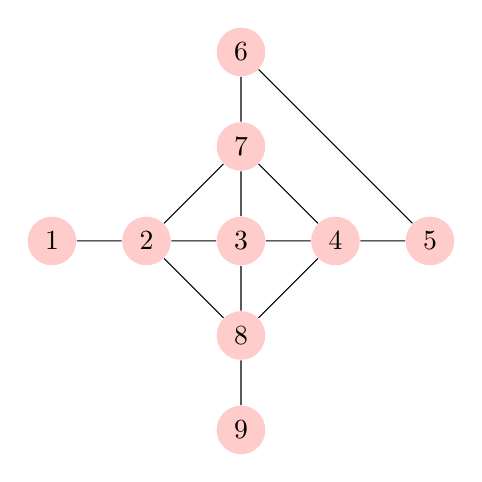
\begin{tikzpicture}
  [scale=.6,auto=left,every node/.style={circle,fill=red!20}]
  \node (n1) at (1,7) {1};
  \node (n2) at (3,7)  {2};
  \node (n3) at (5,7)  {3};
  \node (n4) at (7,7) {4};
  \node (n5) at (9,7)  {5};
  \node (n6) at (5,11)  {6};
   \node (n7) at (5,9) {7};
   \node (n8) at (5,5) {8};
   \node (n9)  at (5,3) {9};
  \foreach \from/\to in {n1/n2,n2/n3,n3/n4,n4/n5,n6/n7,n7/n3,n3/n8,n8/n9,n2/n7,
  n4/n7,n4/n8,n8/n2,n6/n5}
    \draw (\from) -- (\to);

\end{tikzpicture}
\caption{Example graph with nine vertices and 13 edges}\label{4g2}
\end{center}
\end{figure}

Ajur stood perplexed. He tried to reason out an approach he could take, saying out loud, ``Not all of the vertices have an even degree, so that means there is no closed Eulerian walk.''  He studied the graph further.  ``But seven of the nine vertices \textit{do} have an even degree. Vertices~1 and~9 both have an odd degree of~1, so they would definitely be the start and end vertices.''

Rishnak was pleased.

Ajur continued, ``Let me look for cycles.  I see cycles $(2,3,7)$, $(7,6,5,4)$, and $(3,4,8)$, none of which have any edge in common. Aha, I think I got it. I can combine the cycles.''

Ajur excitedly drew a graph in the dirt [Figure~\ref{4g25}], again using arrows to show the path to follow. ``The Eulerian walk is then $1-(1,2)-2-(2,3)-3-(3,4)-4-(4,8)-8-(8,3)-3-(3,7)-7-(7,6)-6-(6,5)-5-(5,4)-4-(4,7)-7-(7,2)-2-(2,8)-8-(8,9)-9$ or we can just say~$(1,2,3,4,8,3,7,6,5,4,7,2,8,9)$.''

Ajur added again that there was no closed Eulerian walk in the graph because not all of the vertices had an even degree. But an Eulerian walk can start from a vertex with an odd degree and then end at a vertex with an odd degree.

\begin{figure}
\begin{center}
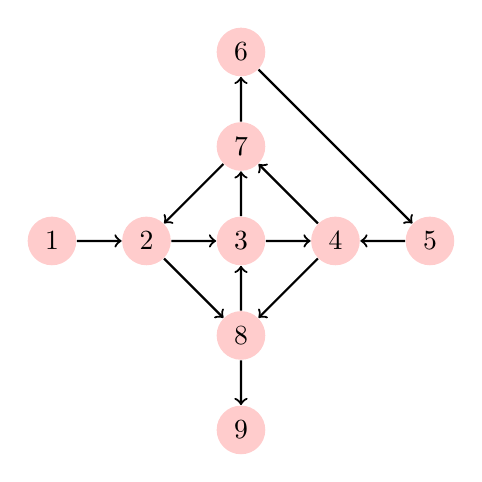
\begin{tikzpicture}
  [scale=.6,auto=left,every node/.style={circle,fill=red!20}]
  \node (n1) at (1,7) {1};
  \node (n2) at (3,7)  {2};
  \node (n3) at (5,7)  {3};
  \node (n4) at (7,7) {4};
  \node (n5) at (9,7)  {5};
  \node (n6) at (5,11)  {6};
   \node (n7) at (5,9) {7};
   \node (n8) at (5,5) {8};
   \node (n9)  at (5,3) {9};
 \path [->,draw,thick] 
  (n1) edge  (n2)
  (n2) edge (n3)
  (n3) edge (n4)
  (n4) edge (n8)
  (n8) edge (n3)
  (n3) edge (n7)
  (n7) edge (n6)
  (n6) edge (n5)
  (n5) edge (n4)
  (n4) edge (n7)
  (n7) edge (n2)
  (n2) edge (n8)
  (n8) edge (n9)
;
\end{tikzpicture}
\caption{Eulerian walk $(1,2,3,4,8,3,7,6,5,4,7,2,8,9)$ from vertex~1 to vertex~9 of the graph shown in Figure~\ref{4g2}}\label{4g25}
\end{center}
\end{figure}

Rishnak said, ``Exactly right. There are exactly two such vertices with odd degrees, and all other vertices must have even degrees. All other vertices become intermediate vertices in the Eulerian walk, meaning that for every edge coming into the vertex there is a corresponding edge leaving that vertex.''

Rishnak asked Ajur how he would modify the original graph [Figure~\ref{4g2}] to have a closed Eulerian walk.

Ajur reasoned this out quickly. He said, ``There are exactly two vertices with odd degrees, namely vertices~1 and~9. If we were to add an edge between these two vertices, then every vertex would have an even degree and a closed Eulerian walk would be possible.''\index{closed Eulerian Walk}

He drew the graph in the dirt [Figure~\ref{4g255}]. ``The closed Eulerian walk would be $(1,2,3,4,8,3,7,6,5,4,7,2,8,9,1)$.''

\begin{figure}
\begin{center}
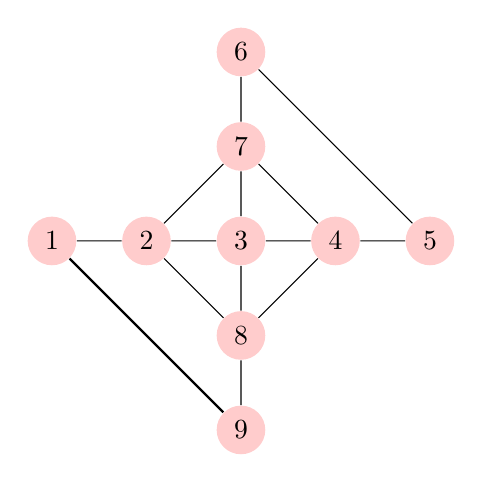
\begin{tikzpicture}
  [scale=.6,auto=left,every node/.style={circle,fill=red!20}]
  \node (n1) at (1,7) {1};
  \node (n2) at (3,7)  {2};
  \node (n3) at (5,7)  {3};
  \node (n4) at (7,7) {4};
  \node (n5) at (9,7)  {5};
  \node (n6) at (5,11)  {6};
   \node (n7) at (5,9) {7};
   \node (n8) at (5,5) {8};
   \node (n9)  at (5,3) {9};
  \foreach \from/\to in {n1/n2,n2/n3,n3/n4,n4/n5,n6/n7,n7/n3,n3/n8,n8/n9,n2/n7,
  n4/n7,n4/n8,n8/n2,n6/n5}
    \draw (\from) -- (\to);
\path[thick] (n1) edge (n9);
\end{tikzpicture}
\caption{The graph from Figure~\ref{4g2} with additional edge~$(1,9)$ enabling closed Eulerian walk $(1,2,3,4,8,3,7,6,5,4,7,2,8,9,1)$}\label{4g255}
\end{center}
\end{figure}

Rishnak smiled. ``Let's go back to this first graph.'' With a flash of his hands, the graph formed in front of him [Figure~\ref{4g1}]. ``How would you modify this graph to have a closed Eulerian walk?''

Ajur now had a problem. The two vertices with odd degrees---vertices~2 and~4---already had an edge between them. He said, ``I don't think we can do it.''

Rishnak said, ``Have you ever heard of a \textit{multigraph}?''

Ajur shook his head.

Rishnak continued, ``In a multigraph, there can be more than one edge between any pair of vertices.''

Ajur pondered this for a moment, then said, ``Oh, I can add another edge between vertex~2 and vertex~4 to get a closed Eulerian walk''---he hurriedly drew a new graph [Figure~\ref{4g155}]---``it's $(2,3,4,1,2,4,2)$.''
%Ajur added that if a graph is not connected, there is neither Eulerian walk nor a closed Eulerian walk (as there is no walk from some vertex to some other vertex - In an Eulerian walk,.

\begin{figure}
\begin{center}
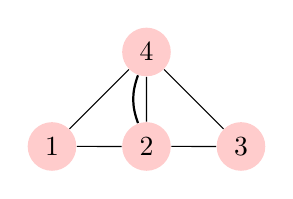
\begin{tikzpicture}
  [scale=.6,auto=left,every node/.style={circle,fill=red!20}]
  \node (n1) at (1,7) {1};
  \node (n2) at (3,7)  {2};
  \node (n3) at (5,7)  {3};
  \node (n4) at (3,9)  {4};

  \foreach \from/\to in {n1/n2,n2/n3,n2/n4,n1/n4,n3/n4}
    \draw (\from) -- (\to);
\path[thick] (n2) edge[bend left=20] (n4);
\end{tikzpicture}
\caption{The graph from Figure~\ref{4g1} with additional edge~$(2,4)$ added to form a multigraph with closed Eulerian walk~$(2,3,4,1,2,4,2)$}\label{4g155}
\end{center}
\end{figure}

Rishnak asked Ajur whether he knew about directed graphs.\index{directed graph}

Ajur nodded and said, ``In a directed graph, an edge~$(x,y)$ only goes from vertex~$x$ to vertex~$y$. I mean it doesn't also go back from vertex~$y$ to vertex~$x$.'' He drew an example graph to show this [Figure~\ref{4g5}].

Rishnak said, ``Right. And instead of talking about the degree of a vertex, we then have an \textit{in-degree} and an \textit{out-degree} of a vertex. The number of edges coming into a vertex is the in-degree of that vertex, while the number of edges going out of a vertex is the out-degree.''

Rishnak drew a new graph in a dazzling display of light [Figure~\ref{4g5}], then said, ``In this directed graph, vertex~1 has an in-degree of~2 and an out-degree of~1. Vertex~3 has an in-degree  and an out-degree~1, same with vertex~4. And a directed graph is said to be \textit{strongly connected} if there is a directed path from every vertex to every other vertex. This example graph is indeed strongly connected.''

Ajur marveled at the graph in front of him.  He said, ``And an Eulerian walk can only exist in a strongly connected directed graph, right?''

Rishnak said, ``Precisely.''

\begin{figure}
\begin{center}
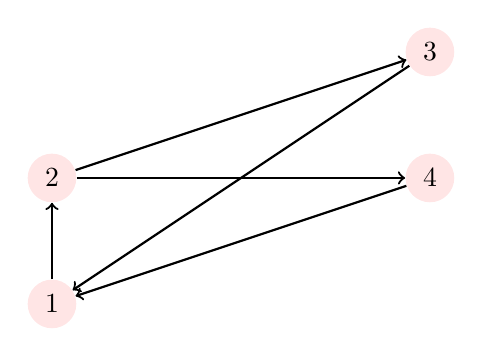
\begin{tikzpicture}
  [scale=.8,auto=left,every node/.style={circle,fill=red!10}]
  \node (n1) at (1,7) {1};
  \node (n2) at (1,9)  {2};
  \node (n3) at (7,11)  {3};
  \node (n4) at (7,9) {4};
 \path[->, draw,thick] 
        (n1) edge (n2)
         (n3) edge (n1)
        (n2) edge (n3)
        (n2) edge (n4)
        (n4) edge  (n1);

\end{tikzpicture}
\caption{Example directed graph with four vertices and five directed edges}\label{4g5}
\end{center}
\end{figure}


Anticipating Rishnak's next question, Ajur said that there was no closed Eulerian walk in this directed graph because there was no way to traverse each edge exactly once and also start and end on the same vertex.

Rishnak said, ``Is there an Eulerian walk from vertex~2 to vertex~1?''

Ajur thought about this, remembering he could try tracing a path without having to raise his pen (or stick) at any point. He reasoned in a manner similar to what he did before. Ajur said, ``I see the cycle~$(2,3,1,2)$, so if I start at vertex~2, I can write the Eulerian walk as $(2,3,1,2,4,1)$.''

Rishnak smiled, then said, ``How could we have a closed Eulerian walk?''

Ajur said, ``We can't in this graph. To have a closed Eulerian walk, we need a collection of cycles that do not share any edges.''

Rishnak said, ``Correct. That is called an \textit{edge-disjoint cycle}, a cycle in which no edge is common. In such a case, the in-degree of each vertex must be the same as its out-degree.''

Ajur nodded and said, ``I see! This is similar to the condition for an undirected graph in which a closed Eulerian walk can only exist if the degree of each vertex is even.''

Rishnak nodded. ``Keep going.''

Ajur said, ``For an Eulerian walk in a directed graph, it has to start from a vertex with an out-degree that is one greater than its in-degree. And it must end at a vertex with an in-degree that is one greater than its out-degree.''

Rishnak said, ``Exactly. And for all other vertices, the in-degree must equal the out-degree.''

It was getting late, but Rishnak wanted to share more about how one could use Eulerian walks---and he wanted to keep Ajur interested. ``Consider the following problem. Let's say you want to construct a string of zeros and ones such that all four of the possible two-bit strings occur as a substring. Note that there are exactly four two-bit strings consisting of zeros and ones, namely~$00$, $01$, $10$, and~$11$. As an example, the string~$00110$ contains all four of these two-bit substrings.''

Ajur nodded, following Rishnak so far anyways.

Rishnak continued, ``Suppose instead, we wanted to build a \textit{circular} string that contained all possible two-bit sub-strings. Such a string is known as a De~Bruijn sequence. \index{De~Bruijn sequence} And this problem is actually closely related to constructing a closed Eulerian walk. Have a look at this directed graph''---he flashed a new graph [Figure~\ref{4g55}] in front of Ajur---``If we construct an Eulerian walk on this directed graph, we would get such a string.''

\begin{figure}
\begin{center}
\begin{tikzpicture}[shorten >=1pt,node distance=4cm,on grid,auto] 
 
   \node[state] (q_1)  {$0$}; 
   \node[state] (q_2) [below =of q_1] {$1$}; 
    \path[->,draw,thick] 
    
    (q_1) edge [bend left=15] node  {1} (q_2)
          edge [loop above] node {0} ()
    (q_2) edge [bend left=15] node [swap] {0} (q_1) 
          edge [loop below] node {1} ();
   
\end{tikzpicture}
\caption{An Eulerian walk on this directed graph will yield a De~Bruijn sequence, which contains all sub-strings of length~2 over binary alphabet~$\{0,1\}$}\label{4g55}
\end{center}
\end{figure}

Ajur frowned. ``How would that work?''

Rishnak said, ``For this directed graph, there are two vertices with labels~$0$ and~$1$. Each directed edge also has a label, which is added to the generated string when the edge is traversed. And the endpoint of that directed edge is the vertex with the same label.''

Ajur understood. ``I see. But why is there a directed edge with label~0 from vertex~0 to itself that---''

Rishnak chimed in, ``That is called a \textit{self loop}.''

Ajur continued, ``A self loop, okay. If we start at vertex~0, then the idea behind this self loop is to append the edge label~0 to the generated string. And we end up still at vertex~0. Similarly, there is an edge with label~1 from vertex~1 to itself. And there is an edge with label~1 from vertex~0 to endpoint vertex~1, and vice versa.''

Rishnak nodded and said, ``Yes. Notice that each vertex has an in-degree of~2 and an out-degree of~2. Therefore, we know that this directed graph has a closed Eulerian walk from vertex~0 back to vertex~0---and that walk is~$0110$. Remember that each character comes from an edge label.''

Ajur smiled and said, ``And from this, we get all four substrings of length~2, namely~$01$, $11$, $10$, and~$00$, with that last one generated by taking the last character and the first character since it is a closed walk.''

Rishnak then asked Ajur to construct a De~Bruijn sequence that contained all substrings of length~3.

Ajur thought about this and rephrased the question. ``Do you mean to obtain a string of zeros and ones such that all eight three-bit strings occur as a substring?''

Rishnak nodded and said, ``Right, what would the eight three-bit strings be?''

Ajur knew the answer to be~$000$, $001$, $010$, $011$, $100$, $101$, $110$, and $111$ by counting in binary (base~2).
Ajur continued, ``Okay, I want to construct a graph from which an Eulerian walk would naturally yield such a sequence, right?''

Rishnak nodded.

Ajur worked out the graph in the dirt using his stick, looking for a pattern to follow.
He started with four vertices labeled~$00$, $01$, $10$, and~$11$.
He drew a directed edge from vertex~$00$ to itself with label~0 because if you get a~0, you can append~0 to the vertex label~$00$, then drop the first character. There is also an edge with label~1 from vertex~$00$ to vertex~$01$.

``Aha!'' exclaimed Ajur. ``You said that every vertex must have an out-degree of~2 and an in-degree of~2.''
%%Similarly there is an edge with label 0 from vertex labeled 01 to vertex with label 10. There is an edge with label 1 from vertex labeled 01 to vertex with label 11. 
%\textbf{For the next paragraph you could cut the rest of the description and just go to the graph} We continue to build the graph following the natural pattern. Draw an edge with label 0 from a  vertex labeled 10 to a vertex labeled 00. Draw an edge with label 1 from a vertex labeled 10 to a vertex labeled 01.
%Draw an edge with label 0 from a vertex labeled 11 to a vertex labeled 10. Draw an edge with label 1 from a vertex labeled 11 to itself.
Ajur drew the rest of the directed graph [Figure~\ref{4g6}] with swift strokes of his stick. ``Starting from vertex~$00$, an Eulerian walk could generate~$0-1-0-1-1-1-0-0$ from the edge labels. This walk is also a closed Eulerian walk since we start and end with the same vertex.''

Rishnak tilted his head and said, ``And?''

Ajur continued, ``And from the walk, we end up with all of the strings of length~3 over alphabet~$\{0,1\}$ as substrings of the Eulerian walk.''

Rishnak said, ``Good.''

\begin{figure}
\begin{center}
\begin{tikzpicture}[shorten >=1pt,node distance=4cm,on grid,auto] 
   \node[state] (q_0)   {$10$}; 
   \node[state] (q_1) [above right=of q_0] {$00$}; 
   \node[state] (q_2) [below right=of q_0] {$11$}; 
   \node[state](q_3) [below right=of q_1] {$01$};
    \path[->,draw,thick] 
    (q_0) edge  node {0} (q_1)
          edge [bend left=15] node  {1} (q_3)
    (q_1) edge  node  {1} (q_3)
          edge [loop above] node {0} ()
    (q_2) edge  node [swap] {0} (q_0) 
          edge [loop below] node {1} ()
    (q_3) edge [bend left=15] node [swap] {0} (q_0) 
          edge  node [swap] {1} (q_2);
\end{tikzpicture}
\caption{A closed Eulerian walk on this directed graph will yield a De~Bruijn sequence that contains all substrings of length~3 over binary alphabet~$\{0,1\}$}\label{4g6}
\end{center}
\end{figure}

Rishnak stretched his arms out wide. He asked, ``Are you sharp enough for something else brand new?''

Ajur smiled and said, ``Yes.''

Rishnak said that another application of the Eulerian walk is in the creation of mazes\index{maze} or labyrinths (as known in Greece) or bhul bulaiyah (as known in India).  He said, ``It is quite easy to enter a maze, but it is difficult to get out of one. In so many stories of old, there are reports of people dying in mazes because they were unable to find their way out. One was the angel Kinaja, who was then a human trapped in a maze. She had figured out how to get out but was too exhausted to walk---and so she died.''

Ajur felt a wave of sadness.

Rishnak quickly said, ``Do not despair, for Kinaja told me that those who studied graph theory and understood Eulerian walks could find their way out of any maze.''

Ajur said that he, too, knew about mazes, having seen a video of a psychology lab experiment with mice running through an elaborate maze. He had also been in a maze as a young boy when his parents took him to a corn field maze.

Eager to show off his knowledge of mazes and poetry, Ajur quoted  Robert Frost's famous poem \textit{The Road not Taken}, which could also be related to traversing a maze---Ajur recited: \begin{quotation}\noindent Two roads diverged in a wood, and I--- \\ 
I took the one less traveled by, \\
And that has made all the difference.
\end{quotation}

\noindent Ajur took a bow.

But Rishnak was getting impatient, as ghosts tend to do, and he wanted to stay focused on the maze and on graphs. Rishnak waved his hands and a glimmering picture of a maze appeared [Figure~\ref{4g7}].

\begin{figure}
\begin{center}
\includegraphics{maze11.jpg}
\caption{A simple maze with a start and a goal, with intermediate steps (vertices) marked for clarity}\label{4g7}
\end{center}
\end{figure}

Rishnak said, ``You can construct a graph from this maze by placing a vertex at each place where there is an open space to move or where you have a choice to make, meaning multiple paths you could follow.''
%\textbf{Can you clarify construction of the maze in this text?}

Ajur gazed at the maze in front of him.

Rishnak continued, ``Join vertices together with an edge if there is a corridor connecting them and there are no vertices already between them. In a maze without any loops, this will result in a tree since no cycles will be present.''

Ajur understood.  He drew a graph [Figure~\ref{4g8}] in the dirt that matched the maze Rishnak showed him.  ``But how does a Eulerian walk make any sense here?''

\begin{figure}
\begin{center}
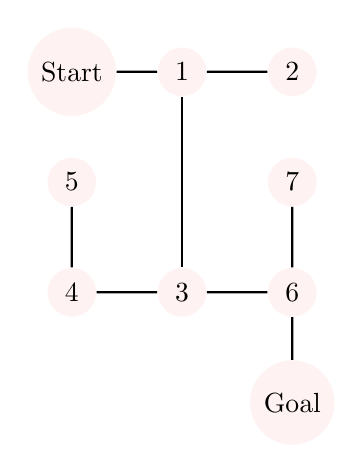
\begin{tikzpicture}
[scale=.7,auto=left,every node/.style={circle,fill=red!5}]
   \node (q_0)   at (1,7) {Start}; 
   \node (q_1) at  (3,7) {1}; 
   \node (q_2) at (5, 7) {2}; 
   \node(q_3) at (3,3) {3};
   \node (q_4) at (1,3) {4};
   \node (q_5) at (1,5) {5};
   \node(q_6) at (5,3) {6};
   \node(q_7) at (5,5) {7};
   \node(q_8) at (5,1) {Goal};
    \path[-,draw,thick] 
    (q_0) edge   (q_1)
    (q_1) edge (q_2)
    (q_1) edge (q_3)
    (q_3) edge  (q_4)
    (q_4) edge (q_5)
    (q_3) edge (q_6)
    (q_6) edge (q_7)
    (q_6) edge (q_8);

\end{tikzpicture}
\caption{A graph (tree actually) corresponding to the maze shown in Figure~\ref{4g7}}\label{4g8}
\end{center}
\end{figure}

Rishnak smiled, happy to see Ajur's desire to learn.  Rishnak said, ``You can make this graph Eulerian by traversing each edge twice. Each time you traverse an edge, you leave a bread crumb to mark it. Once you reach a dead end, you turn back. And if an edge has two bread crumbs, that means you do not traverse that edge any more.''

Rishnak's smile broadened as he continued, ``This was precisely the strategy Kinaja described to me for how to get out of a maze. In the beginning, all of the paths are free of bread crumbs. Whenever one takes a path (if there is one available to take that has no bread crumbs), you mark the edge with a bread crumb. And if there are no paths available without any bread crumbs, you take the path in which there is only one bread crumb present, placing bread crumbs as you go. Eventually you will reach the end goal as there is an Eulerian walk present in the underlying graph of the maze.''

Ajur said, ``Let me see if I understand.'' He drew another maze in the dirt, then drew the graph \textit{inside the maze} [Figure~\ref{4g9}]. ``Like this?''

Rishnak beamed.  ``Precisely.''

\begin{figure}
\begin{center}
\includegraphics[width=0.7\textwidth]{anothermaze.jpg}
\caption{A maze with a start and a goal, with the corresponding graph representation drawn inside the maze}\label{4g9}
\end{center}
\end{figure}

\subsection*{Question for the fourth day}
Rishnak said, ``The time has come for me to ask you the question for the fourth day.''

Ajur straightened, ready for his question.

Rishnak said, ``It has two parts. Going back to this earlier graph''---he flashed the De~Bruijn sequence graph for substrings of length~3 from earlier [Figure~\ref{4g6}]---``first can you write a string (different than the one we already came up with) that contains all substrings of length~3 over binary alphabet~$\{0,1\}$?''

Ajur nodded.  ``And?''

Rishnak said, ``Second, can you construct a directed graph that will yield a De~Bruijn sequence that contains all substrings of length~4 over the same alphabet?''

\textit{Before you turn the page, try to come up with an answer of your own!}

\newpage
\subsection*{Answer for the fourth day}
For length~3, Ajur used the directed graph in front of him [Figure~\ref{4g6}] and wrote a closed Eulerian walk as $0-0-0-1-0-1-1-1$. ``This one contains all substrings of length~3. Going left to right, they are~$000$, $001$, $010$, $101$, $011$, $111$, $110$, and $100$.''

Rishnak smiled and said, ``Keep going.''

For length~4, Ajur cleared a wide patch in the dirt and drew a new graph [Figure~\ref{4a1}]. Once he was done, he checked to be sure that the graph was Eulerian by verifying that the in-degree and out-degree of each vertex was~2.

``Here is the graph and from this graph''---he traced with his stick---``the sequence is $0-0-0-0-1-0-1-0-0-1-1-0-1-1-1-1$ and it contains all the substrings of length~4, which are~$0000$, $0001$, $0010$, $0101$, $1010$, $0100$, $1001$, $0011$, $0110$, $1101$, $1011$, $0111$, $1111$, $1110$, $1100$, and~$1000$.''

\begin{figure}
\begin{center}
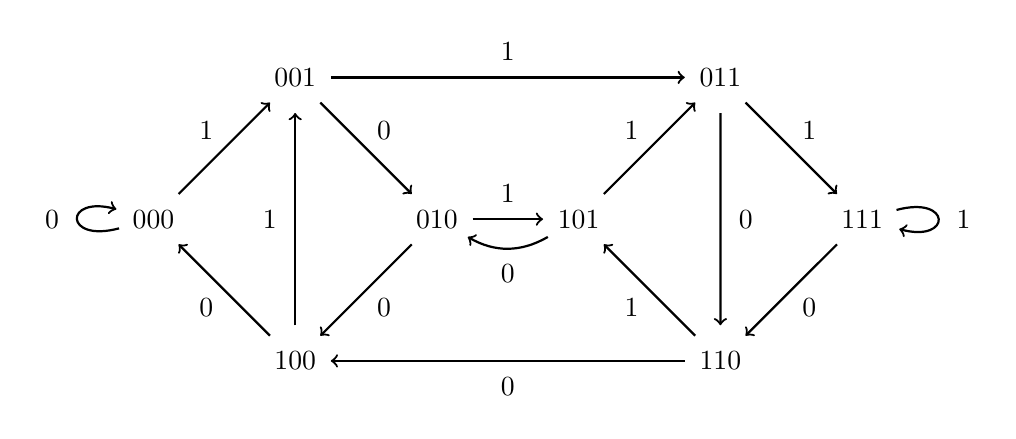
\begin{tikzpicture}
[scale=.6,auto=left,every node/.style={circle}]
   \node (n0)   at (0,0) {000}; 
   \node (n1) at  (3,3) {001}; 
   \node (n2) at (3, -3) {100}; 
   \node (n3) at (6,0) {010};
   \node (n4) at (9,0) {101};
   \node (n5) at (12,3) {011};
   \node(n6) at (12,-3) {110};
   \node(n7) at (15,0) {111};
    \path[->,draw,thick] 
    (n0) edge [loop left] node {0} ()
    (n0) edge  node {1} (n1)
    (n1) edge node {0} (n3)
    (n1) edge node {1} (n5)
    (n2) edge node {1} (n1)
    (n2) edge node {0} (n0)
    (n3) edge node {1} (n4)
    (n3) edge node{0} (n2)
    (n4) edge [bend left] node {0} (n3)
    (n4) edge node {1} (n5)
    (n5) edge node {1}  (n7)
    (n5) edge node {0}  (n6)
    (n6) edge node [bend left] {1} (n4)
    (n6) edge node {0} (n2)
    (n7) edge node {0} (n6)
    (n7) edge [loop right] node {1}()
    ;
  \end{tikzpicture}
\caption{A graph to generate a De~Bruijn sequence of length~4}\label{4a1}
\end{center}
\end{figure}

Rishnak was happy with Ajur's answers. He said, ``Well done.''

Ajur smiled to himself. He was impressed by the power of the Eulerian walk and wanted a walk to be named after him someday, too! The sun was setting and it was time for Ajur and Jura to go home.
